\begin{multicols}{3}
\begin{enumerate}
    \item ~\\
        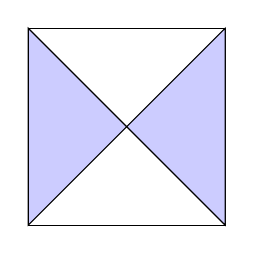
\begin{tikzpicture}[scale=0.5]
        \draw (0,0) rectangle (5,5) ;
        \draw[fill=blue!20] (0,0) -- (5,5) -- (5,0) -- (0,5) -- cycle ;
        \end{tikzpicture}

    \item ~\\
        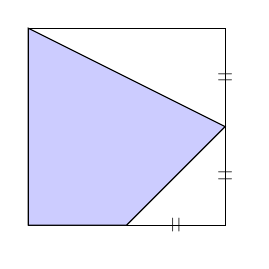
\begin{tikzpicture}[scale=0.5]
        \draw (0,0) --node[near end, sloped]{{\tiny $||$}} (5,0) --node[near start, sloped]{{\tiny $||$}}node[near end, sloped]{{\tiny $||$}} (5,5) -- (0,5) -- cycle;
        \draw[fill=blue!20] (0,0) -- (2.5,0) -- (5,2.5) -- (0,5) -- cycle ;
        \end{tikzpicture}

    \item ~\\
        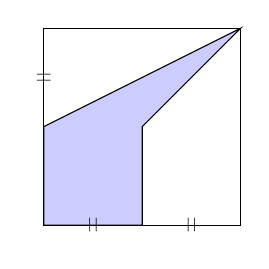
\begin{tikzpicture}[scale=0.5]
        \draw[fill=blue!20] (0,0) -- (2.5,0) -- (2.5,2.5) -- (5,5) -- (0,2.5) -- cycle ;
        \draw (0,0) --node[near start, sloped]{{\tiny $||$}}node[near end, sloped]{{\tiny $||$}} (5,0) -- (5,5) -- (0,5) --node[near start, sloped]{{\tiny $||$}} cycle;
        \end{tikzpicture}
\end{enumerate}
\end{multicols}